\documentclass[12pt]{article}
\title{Mapping rainfall anomalies during the 2015-2016 El Ni{\~n}o event}
\author{P. Krishna Krishnamurthy | UCLA ID: 904723392}
\date{}
\usepackage{graphicx}
\usepackage{float}
\usepackage{textcomp}
\usepackage{listings}
\usepackage{subfig}
\usepackage{hyperref}
\usepackage{color}

%New colors defined below
\definecolor{codegreen}{rgb}{0,0.6,0}
\definecolor{codegray}{rgb}{0.5,0.5,0.5}
\definecolor{codepurple}{rgb}{0.58,0,0.82}
\definecolor{backcolour}{rgb}{0.95,0.95,0.92}

%Code listing style named "mystyle"
\lstdefinestyle{mystyle}{
  backgroundcolor=\color{backcolour},   commentstyle=\color{codegreen},
  keywordstyle=\color{magenta},
  numberstyle=\tiny\color{codegray},
  stringstyle=\color{codepurple},
  basicstyle=\footnotesize,
  breakatwhitespace=false,         
  breaklines=true,                 
  captionpos=b,                    
  keepspaces=true,                 
  numbers=left,                    
  numbersep=5pt,                  
  showspaces=false,                
  showstringspaces=false,
  showtabs=false,                  
  tabsize=2
}

%"mystyle" code listing set
\lstset{style=mystyle}

\begin{document}
\maketitle

\begin{abstract}
There is consensus in the climate science community that El Ni{\~n}o events, periods of anomalously high sea surface temperatures in the Pacific, are associated with disruptions to monsoon patterns which lead to changes in rainfall patterns. The 2015-2016 El Ni{\~n}o episode was an unprecedented event of a scale not seen before, and there is concern that such events may become more frequent under climate change. Understanding rainfall anomalies associated with such large-scale events is the first step towards anticipating potential impacts on vulnerable systems including rain-fed agriculture. Here I utilize remotely-sensed data from the Tropical Rainfall Measurement Mission (TRMM) and the Global Precipitation Measurement Mission (GPM) to illustrate the geographic distributions of rainfall anomalies reported in 2016, at the peak of the recent 2015-2016 Ni{\~n}o event.
\end{abstract}

\section{Introduction}
El Ni{\~n}o events, periods of anomalously high sea surface temperatures in the Pacific, are associated with disruptions to monsoon patterns which lead to changes in rainfall patterns. Weather anomalies from the El Ni{\~n}o Southern Oscillation (ENSO) have historically affected key agricultural producing regions of the world such as Southeast Asia and Southern Africa, and have therefore been associated with food security crises \cite{ray2014effects, iizumi2014impacts}. Analyzing ENSO-induced rainfall anomalies  

The 2015-2016 El Ni{\~n}o episode was an unprecedented event of a scale not seen before, and there is concern that such events may become more frequent under climate change \cite{cai2014increasing}. Understanding rainfall anomalies associated with such large-scale events is the first step towards anticipating potential impacts on vulnerable systems, such as rainfed agriculture. This information can then be used to understand which communities or systems are particularly vulnerable to strong El Ni{\~n}o episodes, and can be used to prepare risk management strategies \cite{wang2017nino}. 

This report illustrates rainfall anomalies reported in 2016 compared to the historical average (1998-2015) using data from the Tropical Rainfall Measurement and the Global Precipitaiton Measurement Missions. The results indicate significant rainfall deficits in southeast Asia, particularly near Indonesia and the Philippines with the highest reductions in December-February. The results indicate potential food security concerns though additional data, such as production estimates and household assessments, are needed to verify the extent of losses. The report is structured as follows: Section 1 highlights the relevance of analyzing rainfall anomalies in the recent El Ni{\~n}o episode, Section 2 presents the data and methods (including annotated codes) used in this analysis, Section 3 assesses the results of the analysis, and Section 4 concludes with a brief summary.

\section{Materials \& Methods}
\subsection{Data}
The TRMM satellite was launched in November 1997 and terminated operations in April 2015. The satellite provided rainfall information at a high spatial resolution (1 degree  by 1 degree) and very high temporal resolution (every 3 hours) for all coordinates between 50\textdegree N and 50\textdegree S. The GPM was launched in February 2014 building on the successes of TRMM and provides compatibility with TRMM datasets. The main difference between the two datasets is that GPM provides data for coordinates between 60\textdegree N and 60\textdegree S. For comparability, results are shown for all coordinates between 50\textdegree N and 50\textdegree S. Data are available for download in 3-hour, 1-day, and 30-day intervals.

Monthly average rainfall rates (measured in terms of mm/hr) were downloaded for the period 1998-2014 from the NASA-TRMM server, and for the period 2015-2016 from the NASA-GPM server. To determine historical rainfall climatology, the average rainfall rate was calculated for the period 1998-2015. A thirty-year dataset is usually considered to be sufficient to establish climatology; unfortunately the historical data are limited so climatology is established using data over a 17-year period. To determine rainfall anomalies in 2016, the difference between the average rainfall values of 2016 and the 17-year historical average was calculated.

However, annual rainfall anomalies only tell part of the story. To better understand the impact of El Ni{\~n}o episodes, it is useful to also consider seasonal rainfall patterns. Seasons were defined as follows: boreal winter (December, January, February; DJF), boreal spring (March, April, May; MAM), boreal summer (June, July, August; JJA), and boreal autumn (September, October, November; SON) following convention in climate science \cite{larkin2005global}. Seasonal anomalies were calculated by first calculating seasonal averages between December 2015 and November 2016, and comparing those to seasonal average rainfall rates between December 1997 and November 2015 (the latter is again considered climatology).      
 
\subsection{Annotated code}
This section includes all annotated codes used for this analysis, including codes to read in precipitation data from an HDF file (Listing 1), calculate the difference between two datasets (Listing 2), code to calculate the average rainfall rates over a prolonged period (Listing 3), and a function to map rainfall data (Listing 4). All of these codes are included in the following github repository: \url{https://github.com/Krishna-K2609/eeb-177-final-project}.

The first function, shown below, takes in a path as an argument and reads in precipitation data, returning a list of rainfall values as well as coordinates. This information generated by this function can then be used to visualize rainfall patterns or perform more sophisticated calculations with numpy.\\

\begin{lstlisting}[language=Python, caption=Reading in precipitation data]
# importing modules and libraries required to read an HDF5 file
import numpy as np
import h5py as h5py

def readPrecip(file_path):
    #this function reads precipitation data from a hdf5 file and returns a list with arrays for each of precipitation, latitude and longitude information
    file = h5py.File(file_path, 'r') 
    # read precipitation data only
    precip = file['Grid/precipitation'][:]
    precip = np.transpose(precip) # transposing the data allows for more sophisticated calculations using numpy functionality.
    # assign geography to values
    theLats = file['Grid/lat'][:]
    theLons = file['Grid/lon'][:]
    return[precip, theLats, theLons]
\end{lstlisting}

The second function, below, takes in four arguments: two files, a title and a destination path. The function further calculates the difference between the two files subtracting the values of the first dataset from the second and produces a map using the specified title and path.\\

\begin{lstlisting}[language=Python, caption=Calculating rainfall anomalies given two datasets]
def precipDifference(file1, file2, title_name, figure_path):
    # the function calculates the difference between file2 and file1
    
    # read precipitation data from file1
    precip1,theLats1,theLons1 = readPrecip(file1)
    
    #repeat for file2
    precip2,theLats2,theLons2 = readPrecip(file2)
    
    # calculate difference
    precipdiff = np.subtract(precip2, precip1)
\end{lstlisting}

The third code consists of a for loop that reads in precipitation data from multiple files and calculates average values over a given period (in this case, the number of months).\\

\begin{lstlisting}[language=Python, caption=Calculating rainfall anomalies given two datasets]
import numpy as np
import h5py as h5py
import os

files = [f for f in os.listdir('/home/eeb177-student/Desktop/eeb177/eeb-177-final-project/data/')]
# obtain all files in a directory

precips = [] # empty list for all precipitation data
for file in files:
    fullpath = '/home/eeb177-student/Desktop/eeb177/eeb-177-final-project/data/'+file # path to files
    precip,TheLats,theLons = readPrecip(fullpath) # using the readPrecip function defined earlier
    precips.append(precip) # appending all rainfall values to the empty list
    
precip_average = np.add(precips)/len(precips) # adding all values in the array and dividing by the length of the list to obtain long-term average
\end{lstlisting}

The final function, highlighted below, takes in an HDF file, a title and destination path as arguments, and generates a map using the title and path specified by the user:\\

\begin{lstlisting}[language=Python, caption=Mapping precipitation data]
# import libraries and modules
from mpl_toolkits.basemap import Basemap, cm
import matplotlib.pyplot as plt
import matplotlib.image as mpimg
import numpy as np
import h5py as h5py

def mapplot(filename, title_name, fig_path):
    #this function maps the results of a HDF5 file. The function takes three arguments (the path to the filename, the desired title for the image, and the path to where the plot should be saved)
    
    # Using the function readPrecip
    precip,theLats,theLons=readPrecip(filename)

    # Plot the figure, define the geographic bounds
    fig = plt.figure(dpi=300)
    latcorners = ([-60,60])
    loncorners = ([-180,180])

    m = Basemap(projection='cyl',llcrnrlat=latcorners[0],\
	urcrnrlat=latcorners[1],llcrnrlon=loncorners[0],\
	urcrnrlon=loncorners[1])

    # Draw coastlinescountry boundaries, edge of map.
    m.drawcoastlines()
    # m.drawstates() # no need for states for this map
    m.drawcountries()

    # Draw filled contours.
    clevs = np.arange(0,1.26,0.125)

    # Define the latitude and longitude data
    x, y = np.float32(np.meshgrid(theLons, theLats))

    # Mask the values less than 0.
    masked_array = np.ma.masked_where(precip < 0,precip) 

    # Assign color scheme
    cmap = cm.GMT_drywet ## NOTE: The current color scheme is not appropriate for maps showing anomalies; instead "cmap = plt.cm.RdBu" should be used for any visualization of differences in rainfall.

    # Plot the data
    cs = m.contourf(x,y,precip,clevs,cmap=cmap,latlon=True) 
	# reports error due to deprecation but produces map
    parallels = np.arange(-60.,61,20.)
    m.drawparallels(parallels,labels=[True,False,True,False])
    meridians = np.arange(-180.,180.,60.)
    m.drawmeridians(meridians,labels=[False,False,False,True])

    #Set the title and fonts
    plt.title(title_name)
    font = {'weight' : 'bold', 'size' : 6}
    plt.rc('font', **font)

    #Add colorbar
    cbar = m.colorbar(cs,location='right',pad="5%")
    cbar.set_label('mm/h')
    #Save figure in desired path
    plt.savefig(fig_path,dpi=200) 
\end{lstlisting}

The code can be modified so that it takes in precipitation averages or differences calculated through any of the previous functions, rather than a specific file, by returning a "precip" dataset:\\
\begin{lstlisting}[language=Python, caption=Mapping precipitation data]
# import libraries and modules
from mpl_toolkits.basemap import Basemap, cm
import matplotlib.pyplot as plt
import matplotlib.image as mpimg
import numpy as np
import h5py as h5py

def mapplot(precip, title_name, fig_path):
    #this function maps a given "precip" value. The function takes three arguments (a dataset called "precip", the desired title for the image, and the path to where the plot should be saved)
    
    # Reading in coordinates.
    data = h5py.File("/home/eeb177-student/Desktop/eeb177/eeb-177-final-project/data/2015/3B-MO.MS.MRG.3IMERG.20151201-S000000-E235959.12.V03D.HDF5", 'r') # Any file can be used as the geography assignment is identical in all files
    theLats = file['Grid/lat'][:]
    theLons = file['Grid/lon'][:]

    # Plot the figure, define the geographic bounds
    fig = plt.figure(dpi=300)
    latcorners = ([-60,60])
    loncorners = ([-180,180])

    m = Basemap(projection='cyl',llcrnrlat=latcorners[0],\
	urcrnrlat=latcorners[1],llcrnrlon=loncorners[0],\
	urcrnrlon=loncorners[1])

    # Draw coastlinescountry boundaries, edge of map.
    m.drawcoastlines()
    # m.drawstates() # no need for states for this map
    m.drawcountries()

    # Draw filled contours.
    clevs = np.arange(0,1.26,0.125)

    # Define the latitude and longitude data
    x, y = np.float32(np.meshgrid(theLons, theLats))

    # Mask the values less than 0.
    masked_array = np.ma.masked_where(precip < 0,precip) 

    # Assign color scheme
    cmap = cm.GMT_drywet ## NOTE: The current color scheme is not appropriate for maps showing anomalies; instead "cmap = plt.cm.RdBu" should be used for any visualization of differences in rainfall.

    # Plot the data
    cs = m.contourf(x,y,precip,clevs,cmap=cmap,latlon=True) 
	# reports error due to deprecation but produces map
    parallels = np.arange(-60.,61,20.)
    m.drawparallels(parallels,labels=[True,False,True,False])
    meridians = np.arange(-180.,180.,60.)
    m.drawmeridians(meridians,labels=[False,False,False,True])

    #Set the title and fonts
    plt.title(title_name)
    font = {'weight' : 'bold', 'size' : 6}
    plt.rc('font', **font)

    #Add colorbar
    cbar = m.colorbar(cs,location='right',pad="5%")
    cbar.set_label('mm/h')
    #Save figure in desired path
    plt.savefig(fig_path,dpi=200) 
\end{lstlisting}

In addition, for this project a simple shell script was written to enable easier downloading of data. The code can be used to download other NASA datasets:\\
\begin{lstlisting}[language=bash]
#! /bin/bash

wget --content-disposition --load-cookies ~/.urs_cookies --save-cookies ~/.urs_cookies --auth-no-challenge=on --keep-session-cookies -i $1

##$1 is a *.dat file containing links to all desired files
\end{lstlisting}

The code depends on a .netrc file and an empty cookies file that can be created using the following commands in the terminal:
\begin{lstlisting}[language=bash]
cd ~
touch .netrc
echo "machine urs.earthdata.nasa.gov login <username> password <password>" >> .netrc
chmod 0600 .netrc
touch .urs_cookies
\end{lstlisting}


\section{Results}
This study evaluated rainfall anomalies in 2016 compared to the historical average (1998-2015). A comparison of the 2016 and 1998-2015 averages indicates distinct geographical patterns of rainfall distribution (Figure 1). The majority of rainfall occurs in the tropics with a peak in the eastern Indian Ocean and the western Pacific Ocean coinciding with the Indonesian archipelago. Here it is important to note that the maps do not illustrate monthly rainfall variations or inter-annual variability: some regions experience higher (or lower) rainfall volumes during specific months and years.

\begin{figure}[htb]
    \label{fig:averages}
\centering
  \subfloat[Mean monthly rainfall rates (2016)]{%
    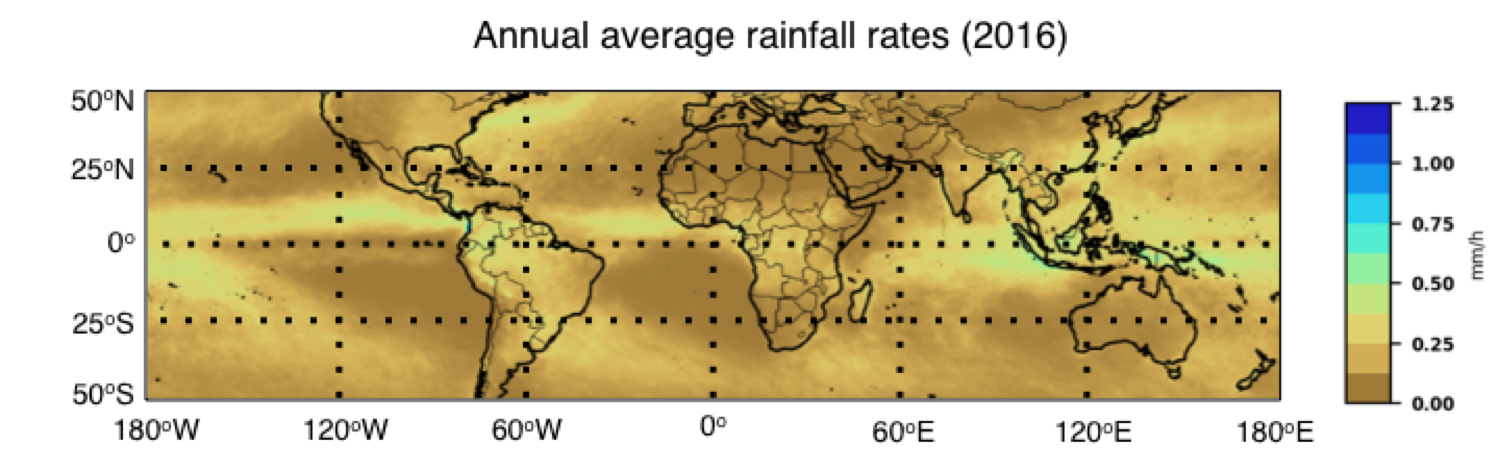
\includegraphics[width=1\textwidth]{figures/2016-ave.png}}\hfill
  \subfloat[Mean monthly rainfall rates (historical average)]{%
    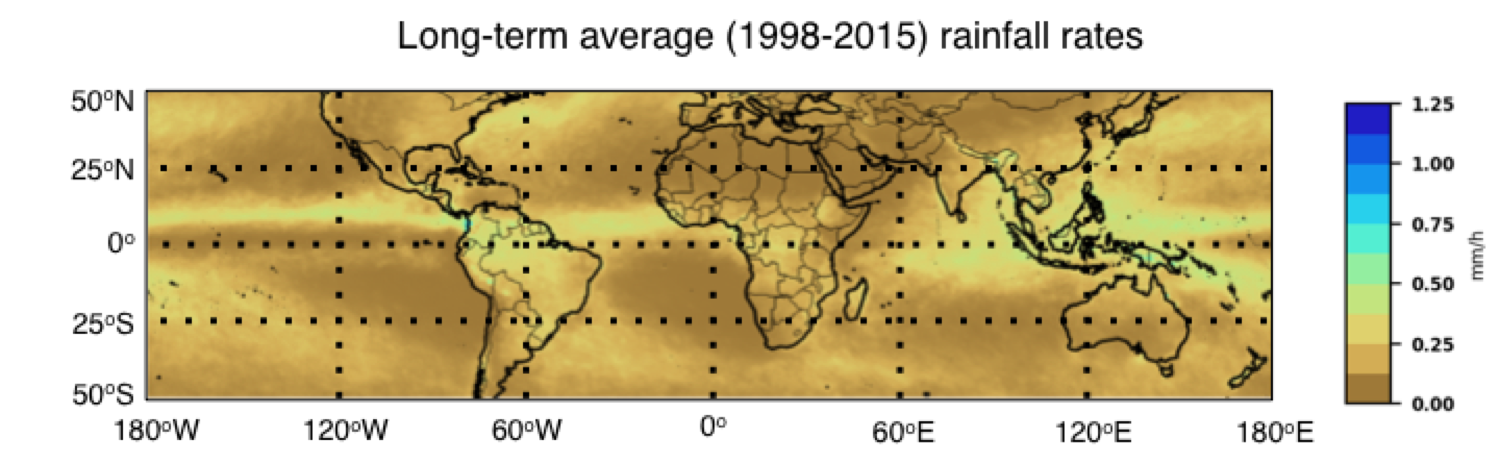
\includegraphics[width=1\textwidth]{figures/lta-ave.png}}\hfill
\caption{Mean monthly rainfall rates for 2016 and the historical average (1998-2015)}
\end{figure}

While the plots are largely similar, there are discernible differences between the two: the western parts of the Indonesian archipelago appear to have received more rainfall than the mainland areas, and the Philippine Islands received substantially lower rainfall in 2016 than in the historical average.

In order to better assess rainfall anomalies, it is useful to consider the differences in rainfall values between 2016 and the historical average (Figure 2). The plot highlights significant rainfall deficiencies in large parts of Indonesia, the Philippines and parts of Sri Lanka. Such anomalies have broader social implications as these countries are major rice producers and exporters; given that paddy production requires significant amounts of water and that irrigation is limited in these countries, reductions in rainfall can result in reduced rice production with food security implications at the national, regional and global levels \cite{zubair2002nino, haile2005weather}. 

\begin{figure}[H]
    \label{fig:lta-difference}
\begin{center}
   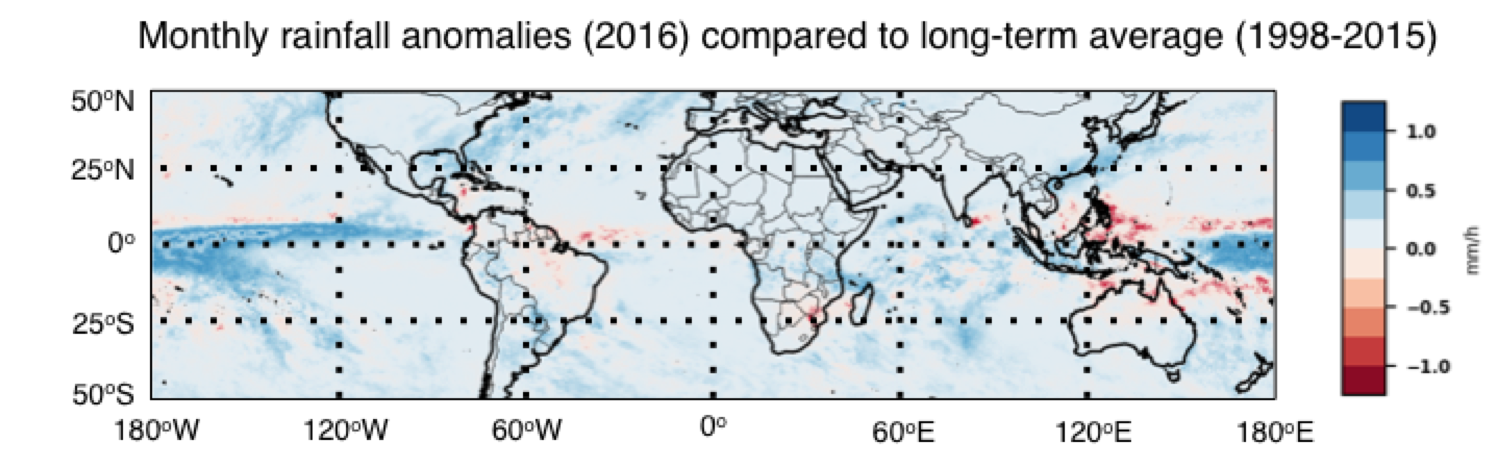
\includegraphics[width=1\linewidth]{figures/lta-diff.png}
\end{center}
\caption{Average monthly rainfall anomalies in 2016 compared to the historical average (1998-2015)}
\end{figure}

However, rainfall anomalies on their own are not enough to cause a food security crisis. Reductions in rainfall during the key growing season are what cause major crop production deficits. It is therefore useful to consider seasonal rainfall anomalies (Figure 3). As shown below, rainfall levels during the period December-February were significantly below the historical average. 

In the Indonesian archipelago, the key agricultural season occurs between December and February. Reductions in rainfall can therefore have significant impacts on national agricultural production \cite{naylor2001using}. Given the lack of irrigation technologies due to the complex topography of the country further exacerbates vulnerability to rainfall deficits. 

In the Philippines, a minor growing season occurs in this period. Paddy produced in this minor rainy season is normally exported; as rice exports contribute significantly to the Philippine economy, lower rice production associated with El Ni{\~n}o can have major deleterious economic consequences \cite{roberts2009nino}.

Sri Lanka also experienced major rainfall deficiencies between December and February. Like the Philippines, Sri Lanka enjoys a second rainy season in the boreal winter which allows for the production of paddy in the north-central region \cite{zubair2002nino}. El Ni{\~n}o-induced reductions in rainfall have had profound impacts on rice production, resulting in price hikes that affect the poorest and most vulnerable communities \cite{zubair2002nino}. 

\begin{figure}[H]
    \label{fig:seasonal-anomalies}
\centering
  \subfloat[Seasonal rainfall anomalies (DJF)]{%
    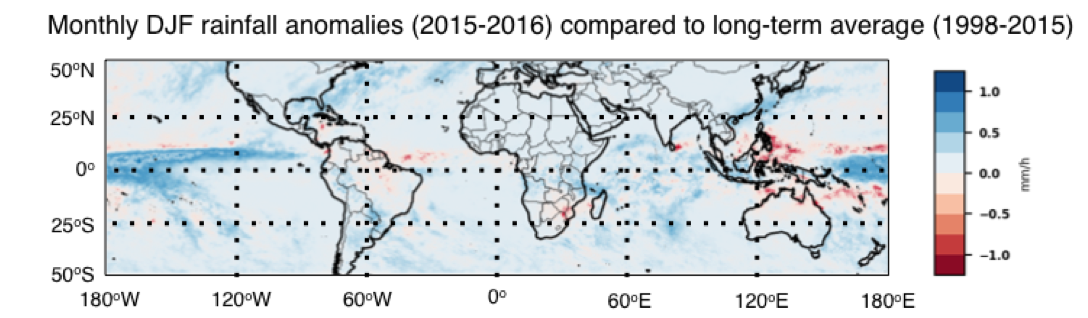
\includegraphics[width=.8\linewidth]{figures/djf-diff.png}}\hfill
  \subfloat[Seasonal rainfall anomalies (MAM)]{%
    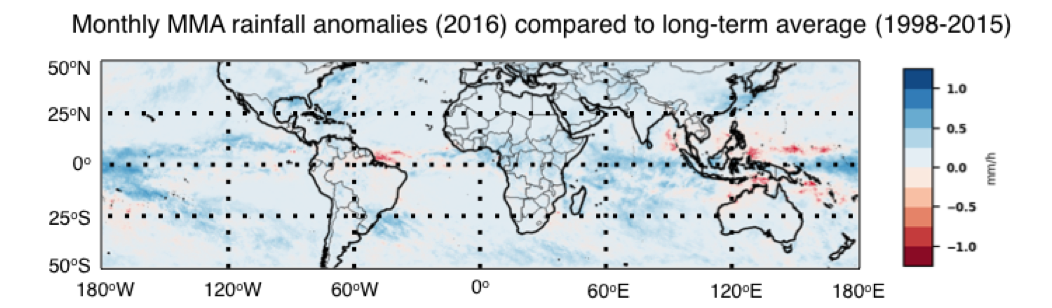
\includegraphics[width=.8\linewidth]{figures/mam-diff.png}}\hfill
  \subfloat[Seasonal rainfall anomalies (JJA)]{%
    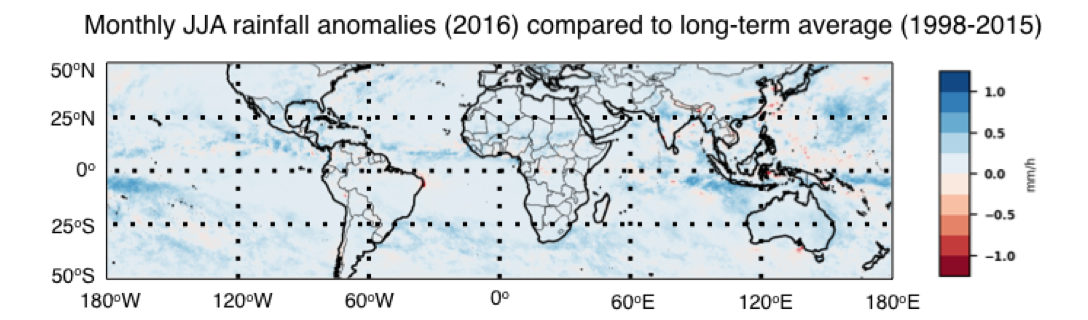
\includegraphics[width=.8\linewidth]{figures/jja-diff.png}}\hfill  
  \subfloat[Seasonal rainfall anomalies (SON)]{%
    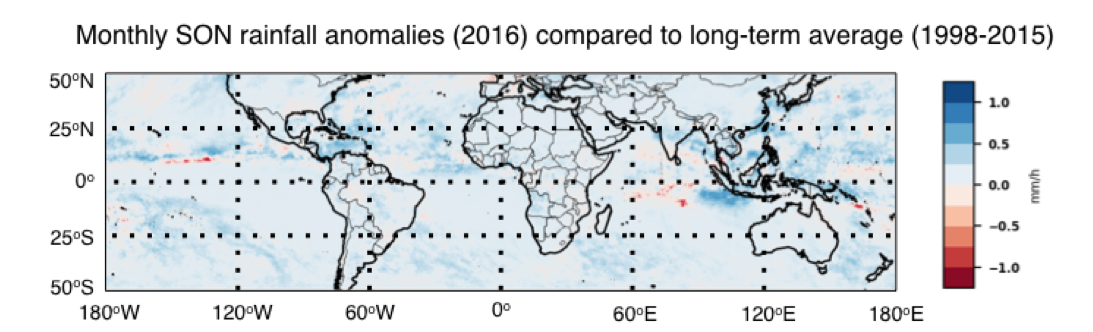
\includegraphics[width=.8\linewidth]{figures/son-diff.png}}\hfill
\caption{Seasonal rainfall anomalies}
\end{figure}


\section{Conclusion}
El Ni{\~n}o Southern Oscillation is an irregular weather phenomenon that can have significant negative impacts on agricultural production in key regions.There is concern among climate scientists that the intensity of ENSO events could become more frequent and intense as sea surface temperatures increase under climate change. The recent 2015-2016 episode, the strongest on record, illustrated the potential rainfall anomalies associated with an intensified Ni{\~n}o event. The maps presented in this report highlighted serious rainfall deficits in south and southeast Asia during a key growing season with potential negative effects on food security and the national economy. To verify the assumption that reduced rainfall resulted in national or regional food security crises, further assessments (of actual crop production, rice imports, and household food security status) are needed. However, the maps presented in this study are useful for the identification of possible areas where additional climate change adaptation and climate risk management strategies are needed to deal with El Ni{\~n}o events.

\bibliography{eeb177.bib}
\bibliographystyle{apalike}

\end{document}
